%!TEX root =  tfg.tex
\chapter{Introduction}

\begin{abstract}
In this chapter, we will explore a little bit about the 
Machine Learning world, the algortihms that people have
been used for years to solve this and other types of problems. A brief summary about the current frameworks that we can use to solve this problem, theirs pros and cons. Finally we are going to explain the problems that we are going to solve. 
\end{abstract}

\section{Artificial Inteligence History}

Deep Learning (DL) has revolutionized industry after industry. People thinks that Deep Learning and Artificial Inteligence (AI) are synonyms, but these words are totally different.
We can define the AI as \emph{the automation of intellectual tasks normally performed by humans}
The AI started in the beginning of the 1957 when John McCarthy held the first academic conference on the subject, the AI machines were able to solve problems that were difficult for humans to solve.

One of the most important AI machines in the history is the Enigma machine built by Alan Turin at the end of World War II. 
This machine could crack in hours entire conversations and text made by the Nazis.

In the early years of AI, a lot of researchers believed that AI could be achieved by hard coding rules. The kind of AI is called symbolic AI and was useful in solving well-defined, logical problems but it was incapable of solving complex problems such as image recognition, object detection, object segmentation, language translation, and natural-languag-understanding.

In order to understand the relationship among AI, ML and DL let's visualize them as concentric circles.


\begin{figure}[H]
\centering
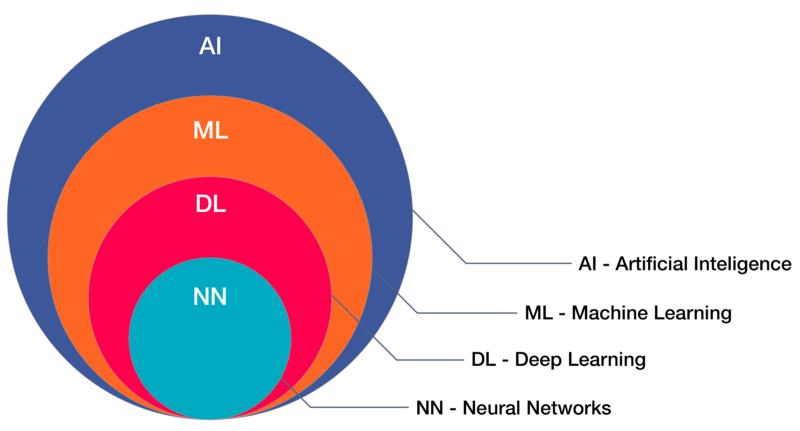
\includegraphics[width=0.8\textwidth]{./figures/ai-ml-dl}
\caption{Representation AI, ML and DL \cite{ai-ml-dl-image}}
\end{figure}

The idea that came first (AI) and the largest one. Then machine learning (ML) which blossomed later), and finally  DL which is driving today's AI explosion (fitting inside both).

\subsection[Machine Learning]{Machine Learning}
Machine Learning (ML) is a sub-field of AI and has become very popular in the last 10 years. AI has a lot of other sub-fields aside from Machine Learning, ML systems are built by showing lots of examples, unlike symbolic AI where we hard code rules to build the system. 

\begin{figure}[H]
\centering
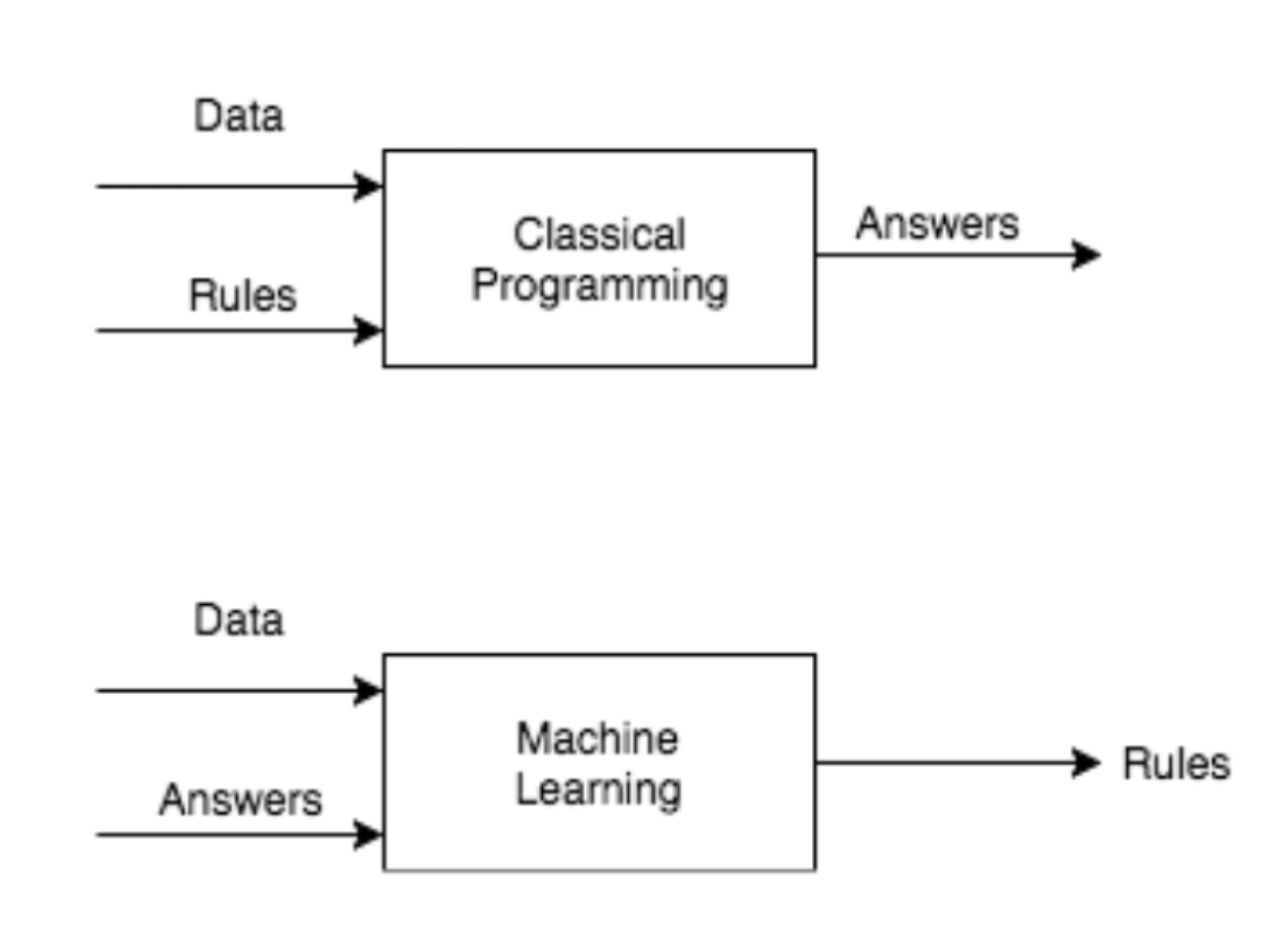
\includegraphics[width=0.8\textwidth]{./figures/ml-structure}
\caption{ML vs Traditional programming}
\end{figure}

At a high level, machine learning systems took at tons of data and come up with rules to predict outcomes for unseen data.
Some examples of machine learning systems in the real life are:

\begin{itemize}
\item Google Photos uses a specific form of machine learning for grouping photos.
\item Recommendations systems which are family of ML algorithms. We can see this kind of recommendations systems in many famous apps like Spotify (music), Netflix (movies) and Amazon (products).
\end{itemize}

\subsection[Deep Learning]{Deep Learning}
Deep Learning is a subfield of ML, that uses specific algorithms in order to predict for example whether an image contains a face or not. It extracts features suach as the first layer detecting edges, the second layer detecting shapes such as noses and eyes and the final layer detecting face shapes or more complex structures.

The use of DL has grown tremendously in the last few years with the rise of GPUs, big data, cloud providers (Amazon Web Services) and frameworks such as Torch, Tensorflow or Pytorch.


\section{State of the art}
\subsection[Neuronal network]{Neuronal network}

A neuronal network is a mathematical model that try to represents how our mind works. The first mathematical model was presented in 1943 called McCulloch-Pitts this model could do several simple tasks. \cite{fsancho}

\begin{figure}[H]
\centering
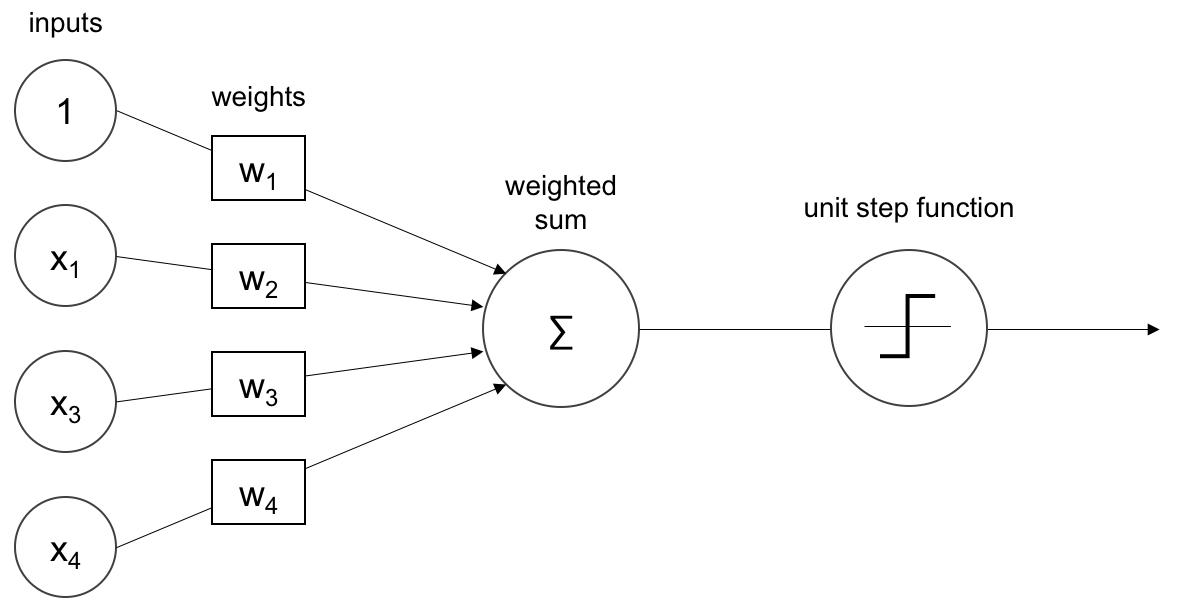
\includegraphics[width=0.8\textwidth]{./figures/perceptron}
\caption{Example of a perceptron \cite{rajalingappaa}}
\end{figure}
	
	
This picture represents a perceptron wich has a set of inputs that are going to be multiplied by their weights.
Then the perceptron will permform a weighted summmation to produce an output. \cite{sagar} Finally the output of the perceptron can be passed through an activation function or transfer function.\cite{rajalingappaa}
The process that the weight of the inputs changes in order to improve the output of the perceptron is called trainning. 

An Artificial Neuronal Netrowk (ANN) is a collection of perceptrons and activation functions. The perceptrons are connected to form hidden layers or units. The hidden units form the nonlinear basis that maps the input layers to output layers in a lower-dimensional space, which is also called artificial neural networks. ANN is a map from input to output. The map is computed by weighted addition of the inputs with biases. The values of weight and bias values along with the architecture are called model.

\begin{figure}[H]
\centering
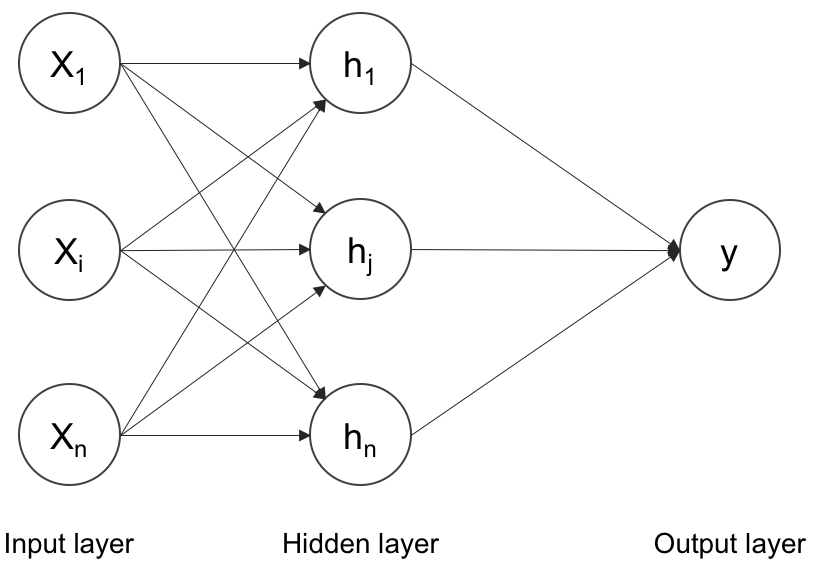
\includegraphics[width=0.8\textwidth]{./figures/ann}
\caption{Example of an Artificial Neuronal Network (ANN) \cite{rajalingappaa}}
\end{figure}
 
The ANN contains several parameters to optimize. The procedure of updating the weights is called backpropagation. The weights are updated from backward based on the error calculated. The procedure to minimize the error is called optimization.

\begin{figure}[H]
\centering
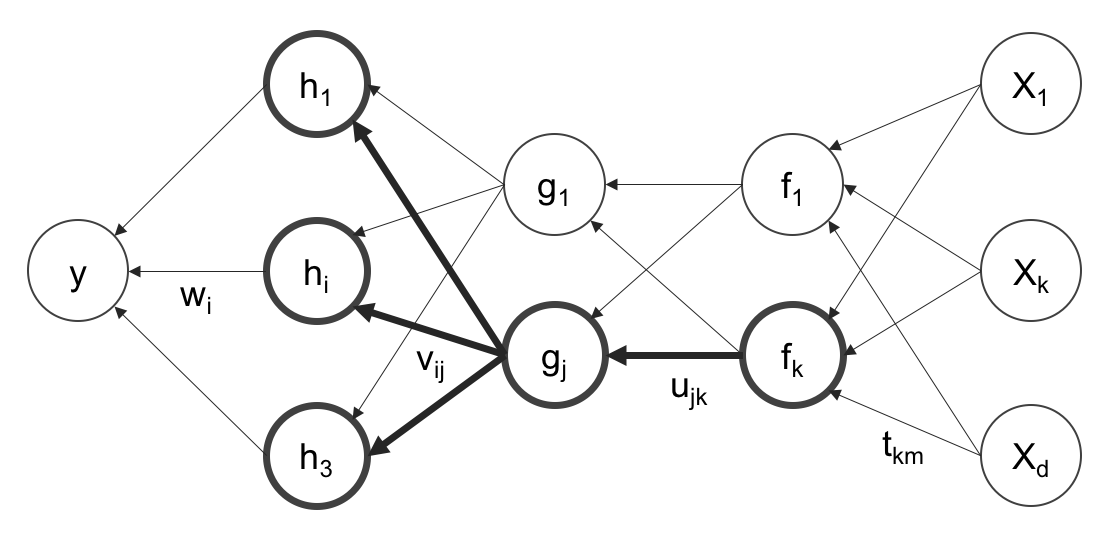
\includegraphics[width=0.8\textwidth]{./figures/backpropagation}
\caption{Example of backpropagation procedure \cite{rajalingappaa}}
\end{figure}

   
A few different ANN models are availables among them the Convolutional Neural Network (CNN) and Recurrent Neural Network (RNN). They have made some revolutionary improvements in the data analysis field. 

\subsection[Unsupervised Pretrained Networks]{Unsupervised Pretrained Networks}

\subsubsection[Autoencoders]{Autoencoders}

Autoencoder is an architecture for unsupervised learning. The main porpouse ot this architecture is to reduce the dimensionality of the dataset and it learns directly from the input data. 
The structure is very simple, the input layer followed by the bottleneck where the encoder and decoder operation are done and finally the output layer that contains the same number of units as the input layer does.\cite{dp4j-deep-learning}

\begin{figure}[H]
\centering
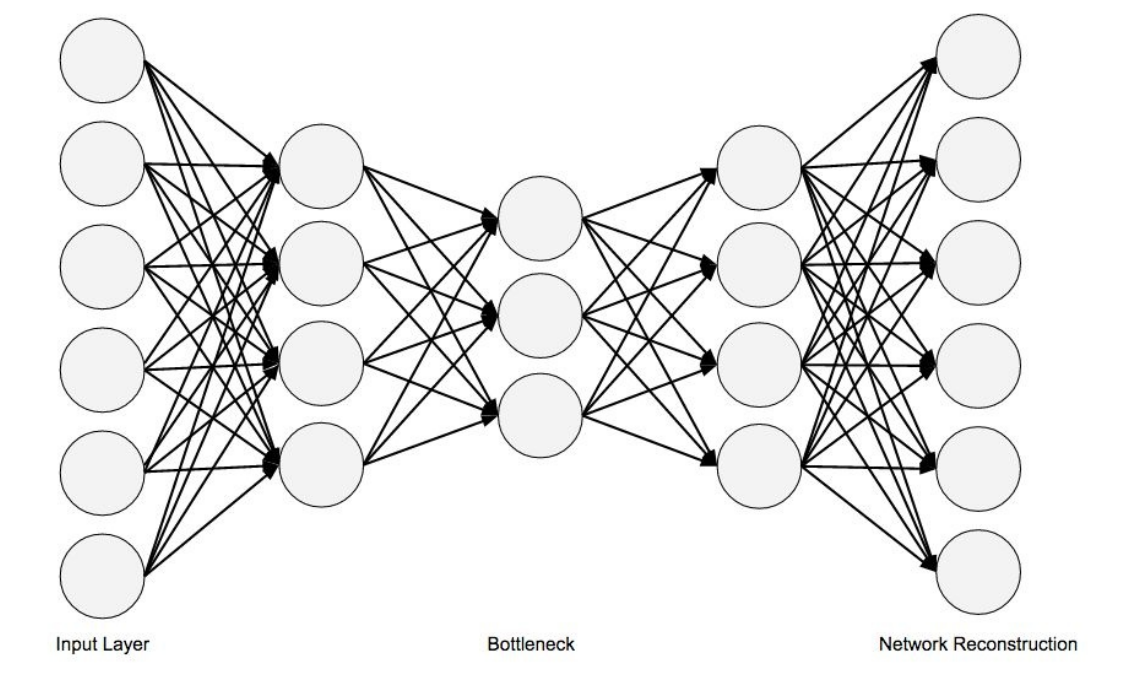
\includegraphics[width=0.8\textwidth]{./figures/autoencoder}
\caption{Example of Autoencoder \cite{dp4j-deep-learning}}
\end{figure}


\subsubsection[Deep Belief Networks]{Deep Belief Networks}
Deep Belief Networks (DBNs) are composed of layer of Restricted Boltzmann Machines (RBMs). In unsupervised learning we use RBMs to extract high-level features from the input data. We discovered that if we let to RBMs to extract this high-level features it progressively can combine nonlinear functions to extract more complex data, to understand better how it works we can see an example with MNIST digits.\cite{dp4j-deep-learning}


\begin{figure}[H]
\centering
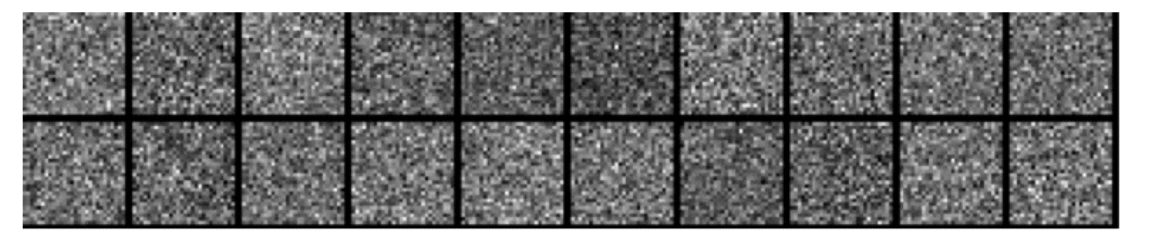
\includegraphics[width=0.8\textwidth]{./figures/rbmm-1}
\caption{Activation render at the beginning of training \cite{dp4j-deep-learning}}
\end{figure}

\begin{figure}[H]
\centering
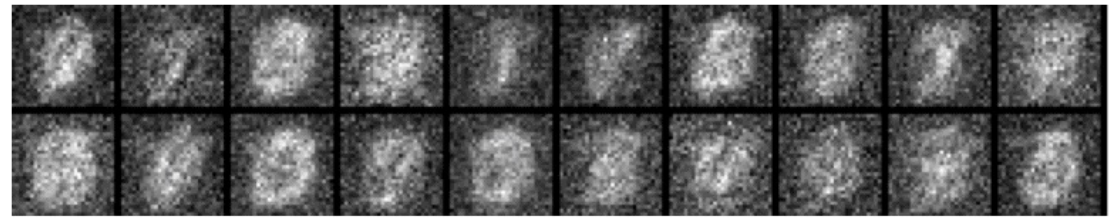
\includegraphics[width=0.8\textwidth]{./figures/rbmm-2}
\caption{Features emerge in later activation render \cite{dp4j-deep-learning}}
\end{figure}

\begin{figure}[H]
\centering
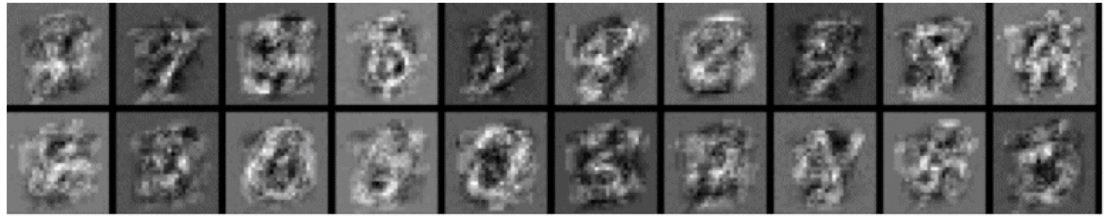
\includegraphics[width=0.8\textwidth]{./figures/rbmm-3}
\caption{Portions of MNIST digits emerge towards end of training \cite{dp4j-deep-learning}}
\end{figure}

\subsubsection[Generative Adversarial Networks]{Generative Adversarial Networks}
The Generative Adversarial Networks is an example of unsupervised learning architecture where we train two models in parallel. Nowdays GANs architecture become really famous to create new images based on other images\cite{dp4j-deep-learning}. 

\begin{figure}[H]
\centering
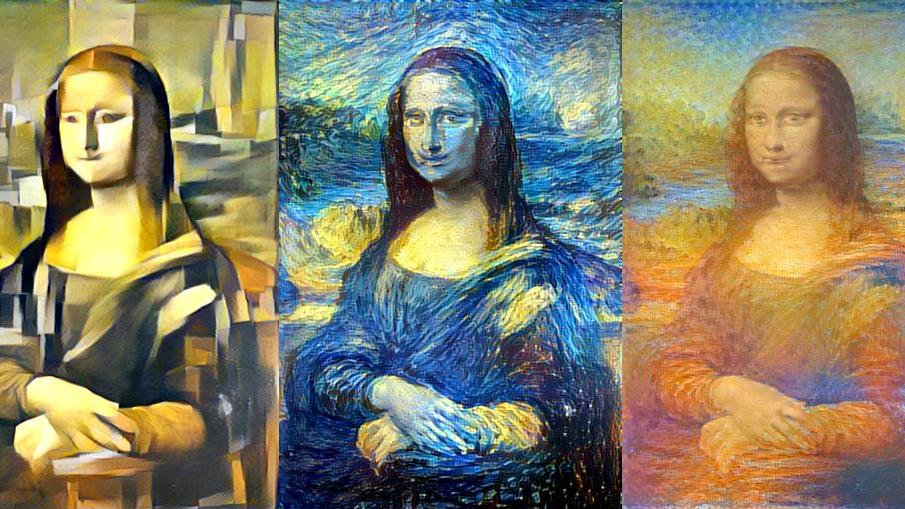
\includegraphics[width=0.8\textwidth]{./figures/monalisa}
\caption{Example of a GAN with The Mona Lisa painting \cite{can-art}}
\end{figure}

GAN is composed by two players, one player (the generator) generates samples that are similar to the trainning data without having access to that data and the second player (the discriminator) examine that samples and determine that data is real or fake.\cite{can-art}


\subsection[Reinforcement Learning]{Reinforcement Learning}

Reinforcement Learning is a subfield of machine learning which addresses
the problem of automatic learning of optimal decisions over time. This is
a general and common problem studied in many scientific and engineering fields.\cite{reinforcement-learning}

Reinforcement Learning (RL) is the third camp and lays somewhere in between full supervision and a complete lack of predefined labels. On the one hand, it uses many well-established methods of supervised learning such as deep neural networks for function approximation, stochastic gradient descent, and backpropagation, to learn data representation.
On the other hand, it usually applies them in a different way. We need an agent that takes actions in some environment.

A good example of this is a robot mouse in a maze, Its environment is a maze with food at some points and electricity at others. The robot
mouse can take actions such as turn left/right and move forward. Finally, at every moment it can observe the full state of the maze to make a 
decision about the actions it may take.
\begin{figure}[H]
\centering
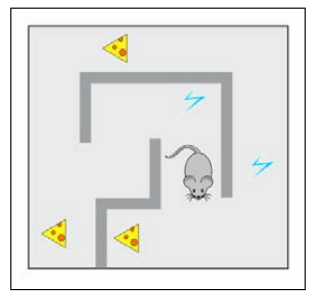
\includegraphics[width=0.5\textwidth]{./figures/robotmouse-maze}
\caption{Example of the Robot Mouse scenario \cite{reinforcement-learning}}
\end{figure}
It is trying to find as much food as  possible, while avoiding an electric shock whenever possible.These food and electricity signals stand as a reward given to the agent by the environment as additional feedback about the agent's actions.


\subsection[Convolutional Neuronal Network (CNN)]{Convolutional Neuronal Network (CNN)}


If we want to use a ANN for images the size of the network will be very large because of the number of neurons and will results an overfitting. Moreover in the case that we want to use big resolution images the size of the network will be huge \cite{rajalingappaa}

The convolutional neuronal network (CNN) is an advance ANN, which allows the network to extract local as well as global features from the data, enhancing the decision-making procedure of the network\cite{abdullah}. Furthermore a CNN that typically has convolutional layers interspersed with pooling (or sub-sampling) layers and then followed by fully connected layers as in a standard multi-layer neural network.\cite{greenspan}

\begin{figure}[H]
\centering
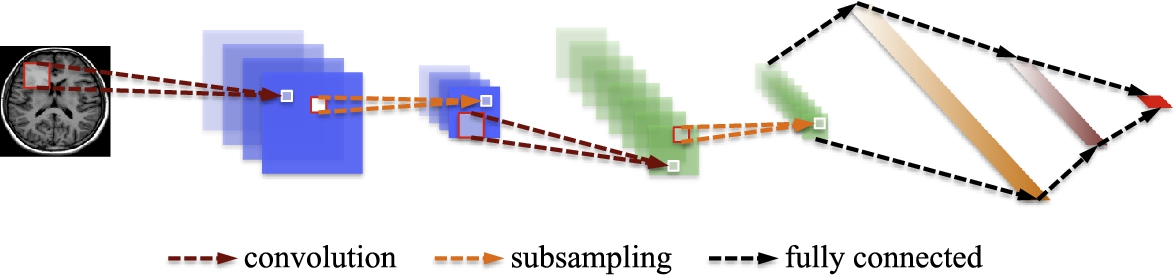
\includegraphics[width=0.8\textwidth]{./figures/cnn}
\caption{An architecture of a convolutional neural network}
\end{figure}

\subsubsection[Convolution]{Convolution}

A convolution is defined as a mathematical operation describing a rule for how to merge two sets of information. \cite{starteddeeplearning}

\begin{figure}[H]
\centering
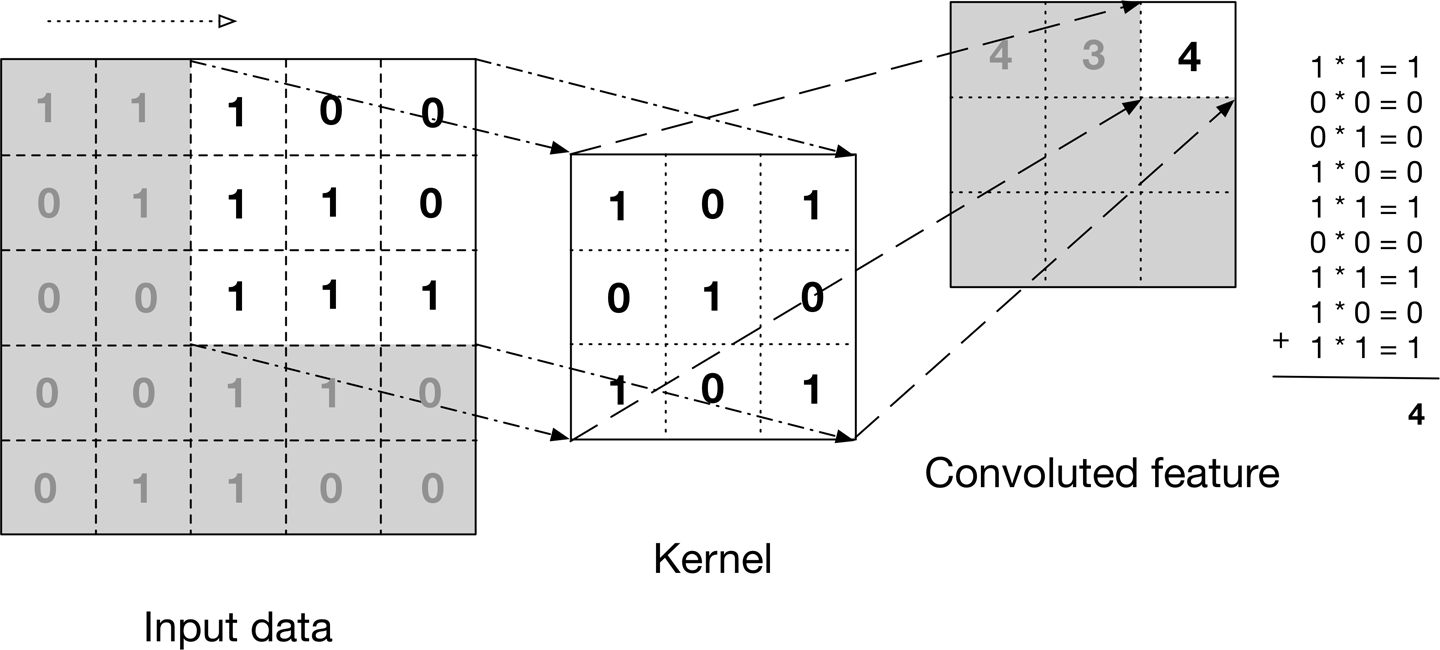
\includegraphics[width=0.8\textwidth]{./figures/convolution}
\caption{The convolution operation \cite{rajalingappaa}}
\end{figure}

The figure ilustrate how the kernel is slid across the input data to produce the convoluted feature (output) data. 

\subsubsection[Pooling]{Pooling}

Usually after the convolution layer we will include a pooling layer to reduce the spatial size \cite{starteddeeplearning} (height and width) for the next layer. The most common pooling operation is max-pooling that reduces the size by a factor of $n^2$ \cite{greenspan} but exists other pooling operations like average-pooling, winner-takes-all pooling \cite{advancesneuralinformation} and stochastic pooling \cite{stochastic}.

\subsubsection[Fully Connected Layers]{Fully Connected Layers}
We use this layer to compute class scores that we’ll use as output of the network. The dimension of the final output will be [1 x 1 x N] where N is the number of classes \cite{starteddeeplearning}. For example in our case the number of classes will be 2 (carcinogenic or  not).


\section{Software}
There are many frameworks to resolve this problem. We are going to explain some for Python and compare them in order to choose the best framework to resolve our problem. 

\subsection[Tensorflow]{Tensorflow}
Tensorflow was created by the IA Google Team. They followed the same structure that Theano library, the engine was written in C/C++ to increase the speed \cite{generalcomparaison}
It support the CPU and GPU operations and you can run with multiple  GPU to optimize your model \cite{tensorflow}. Furthermore this library include a visualization of your model called Tensorboard so you are able to see how is trainning your model for debugging and optimization. Tensorflow is the most famous library for Machine Learning (ML) works but, it's hard to learn and understand how it works in the beginning if we don't have any other experience in ML.


\begin{figure}[H]
\centering
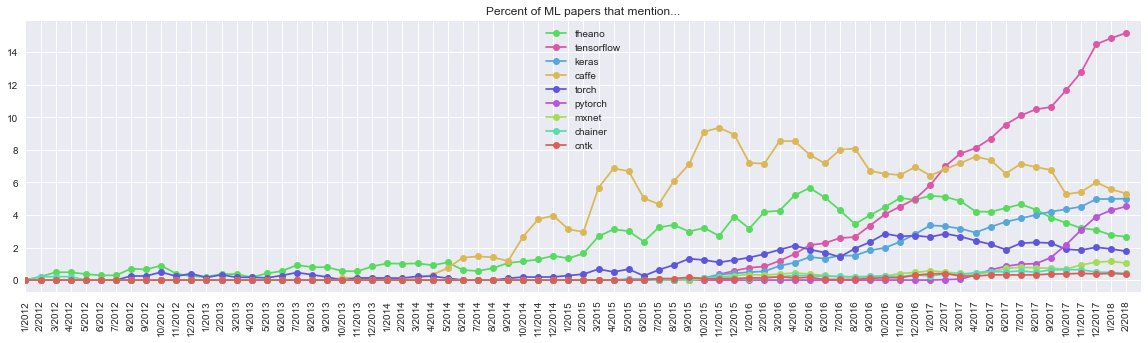
\includegraphics[width=1\textwidth]{./figures/libraries}
\caption{Percent of mentions in ML papers \cite{ml-mentions-image}}
\end{figure}


\subsection[Theano]{Theano}
Maintained by Montréal University group \cite{specificcomparaison} they were the pioneered to use a computational graph that will be use in Tensorflow project \cite{generalcomparaison}. The big cons is for large models Theano will take long time to compute it, also it doesn't support multiple GPU. The error messages can be unhelpful so it will be hard for debugging tasks.

\subsection[Keras]{Keras}
Keras is an easy-to-use Python library \cite{specificcomparaison}
that sits atop Tensorflow and Theano so it took the advantages of both. It has an intuitive and simple API so you can write a model with a few lines of code. Keras is not really flexible and has some problems to use the multi-gpu. 

\subsection[Pytorch]{Pytorch}
The Python version of Torch called Pytorch is an open source project of Facebook created in January 2017. PyTorch has quickly become the favorite among machine-learning researchers, because it allows certain complex architectures to be built easily. \cite{generalcomparaison}. Furthermore the modularity of Pytorch because it's easy to pull someone's code and use  luarocks to install required packages \cite{specificcomparaison}. 

\subsection[H20]{H2O}
It's an open source software platform which core is coded in Java \cite{h20-deeplearning}
H20 is feature-rich, ease of use and it's known for it's R and Spark integration but it provides support to other languages. \cite{h20-comparative-table}
H20 counts with other plugins to create an easy app after train your model (Shinny App).
 
\subsection[DL4J]{DL4J}
DL4J is a JVM-based, industry-focused, commercially supported, distributed deep-learning framework \cite{generalcomparaison}. Python has many scientific environments to work with Deep Learning like Numpy or Theano but DL4J with Java and Scala has several advantages,
Java and Scala are inherently faster than Python. Anything written in Python by itself, disregarding its reliance on Cython, will be slower.
Furthermore the license under DL4J is Apache 2.0 License so anyone is free to make and patents derivate works based on Apache 2.0-licensed code. 

\section[Evaluate the model]{Evaluate the model}
There are many metrics and ways to evaluate the model and check the accuracy. Depends of the scenario we have to use a specific metric or other, there is not exist a metric for all the possibles scenarios. 
The objective of this section is to explain most of the famous metrics for a classification problem.

\subsection[Confusion Matrix]{Confusion Matrix}
This metric is the simplest because it's very easy to use and understand. Each column of the matrix represents the number of predictions for each class, while each row represents the instances in the actual class. One of the benefits of confusion matrices is that they make it easier to see if the system is confusing two classes.

The associated values of a confusion matrix are:

\begin{enumerate}
\item \textbf{True Positives (TP):} test result is one that detects the condition when the
condition is present. Sick people correctly identified as sick.
\item \textbf{True Negative (TN):} test result is one that does not detect the condition when
the condition is absent. Healthy people correctly identified as healthy
\item \textbf{False Positive (FP):} test result is one that detects the condition when the
condition is absent. Healthy people incorrectly identified as sick
\item \textbf{False Negative (FP):} test result is one that does not detect the condition when
the condition is present. Sick people incorrectly identified as healthy
\end{enumerate}


Let's see an example of the confusion matrix to understand how it works. 
The scenario is a dog vs cat classification and the results are the following:
\begin{table}[H]
\centering
\begin{tabular}{llll}
\multicolumn{2}{l}{}                   & \multicolumn{2}{l}{Actual Class}  \\
\multicolumn{2}{l}{}                   & Cat & Dog                         \\
\multirow{2}{*}{Predicted Class} & Cat & 5   & 2                           \\
                                 & Dog & 3   & 3                          
\end{tabular}
\end{table}

\subsubsection[Sensitive]{Sensitive}
Measures the ability of a test to detect the condition when the condition is present.
\[ Sensitive = TP/(TP+FN) \]
In our cat classificator the sensitive is:
\[ Sensitive = 5/(5+3) = 0.625 \]

\begin{figure}[H]
\centering
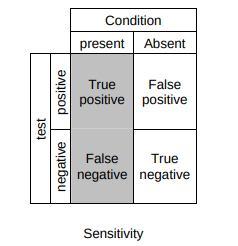
\includegraphics[width=0.3\textwidth]{./figures/Sensitive}
\caption{Calculate the Sensitive}
\end{figure}

\subsubsection[Specificity]{Specificity}
Measures the ability of a test to correctly exclude the condition (not detect the condition) when the condition is absent.
\[ Specificity  = TN/(TN+FP) \]
In our cat classificator the specificity is:
\[ Specificity = 3/(3+2) = 0.6 \]

\begin{figure}[H]
\centering
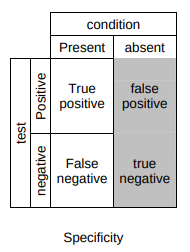
\includegraphics[width=0.3\textwidth]{./figures/Specificity}
\caption{Calculate the Specificity}
\end{figure}

\subsubsection[Predictive value positive]{Predictive value positive}
Measures the proportion of positives that correspond to the presence of the condition.
\[ PVP  =  TP/(TP+FP) \]
In our cat classificator the predictive value positive is:
\[ PVP = 5/(5+2) = 0.714 \]

\begin{figure}[H]
\centering
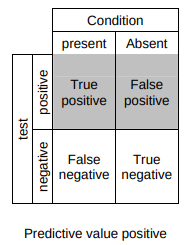
\includegraphics[width=0.3\textwidth]{./figures/PredictiveValuePositive}
\caption{Calculate the Predictive Value Positive}
\end{figure}


\subsubsection[Predictive value negative]{Predictive value negative}
Measures is the proportion of negatives that correspond to the absence of the condition. 
\[ PVN =  TN/(TN+FN) \]
In our cat classificator the predictive value negative is:
\[ PVN = 3/(3+3) = 0.5 \]

\begin{figure}[H]
\centering
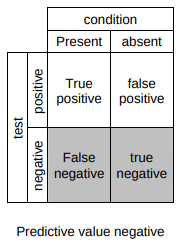
\includegraphics[width=0.3\textwidth]{./figures/PredictiveValueNegative}
\caption{Calculate the Predictive Value Negative}
\end{figure}

\subsection[The Area Under an ROC Curve]{The Area Under an ROC Curve}

The area under the ROC curve ( AUC ) is a measure of how well a parameter can distinguish between two diagnostic groups (diseased/normal). 

\begin{figure}[H]
\centering
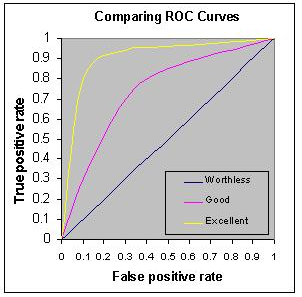
\includegraphics[width=0.3\textwidth]{./figures/ROC}
\caption{Examples of differents ROC curves \cite{area-roc-curve}}
\end{figure}

It's a famous metric in the health scenario, the accuracy is measured by the area under the ROC curve. An area of 1 represents a perfect test; an area of .5 represents a worthless test \cite{area-roc-curve}. A rough guide for classifying the accuracy of a diagnostic test is the traditional academic point system:

\begin{enumerate}
\item \textbf{.90 - 1} Excellent (A)
\item \textbf{.80 - .90} Good (B)
\item \textbf{.70 - .80} Fair (C)
\item \textbf{.60 - .70} Poor (D)
\item \textbf{.50 - .60} Fail (F)
\end{enumerate}


\section[Architectures]{Architectures}

Neural network can be compared with lego blocks, where you can build almost any simplex to complex structures. Actually, most of the famous architectures have been discovered during the Imagenet challenge, this challenge evaluates algorithms for object detection and image classification at large scale\cite{architectures}.

Depends of the task that we want to solve we have to use a type of architecture or other. The main types of tasks that computer vision can be categorised in are as follows:


\begin{figure}[H]
\centering
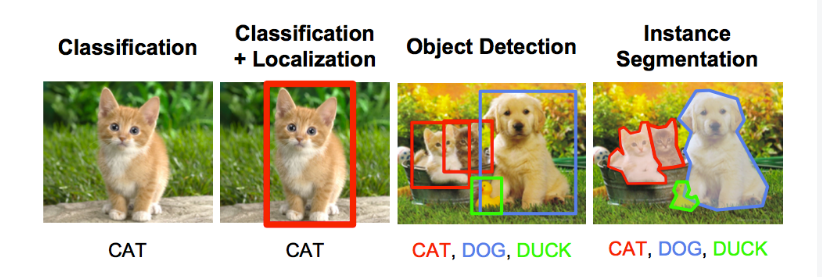
\includegraphics[width=0.7\textwidth]{./figures/Tasks-Architectures}
\caption{Examples of the main types of task in computer vision \cite{architectures}}
\end{figure}

\begin{enumerate}
\item \textbf{Object Recognition / Classification.} In object recognition, the goal is to identify the class givin a raw image.
\item \textbf{Classification + Localisation.} - In this one we have to identify the class and find the location of that object in the raw image.
\item \textbf{Object Detection.} The task is to identify where in the image does the objects lies in. 
\item \textbf{Image Segmentation.} It's a bit sophisticated task, where the objective is to map each pixel to its rightful class.
\end{enumerate}

\subsection[AlexNet]{AlexNet}

\begin{figure}[H]
\centering
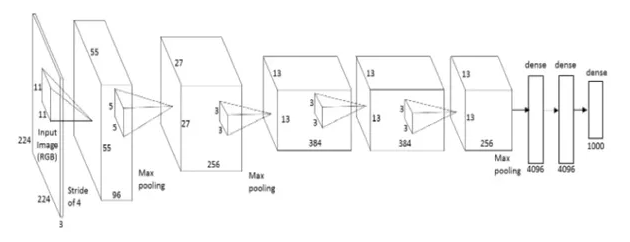
\includegraphics[width=0.6\textwidth]{./figures/Alexnet}
\caption{AlexNet Architecture}
\end{figure}

It's the first deep architecture created by Geoffrey Hinton and his colleagues. When broken down, AlexNet seems like a simple architecture with convolutional and pooling layers one on top of the other, followed by fully connected layers at the top. This is a very simple architecture, which was conceptualised way back in 1980s.

\subsection[VGG Net]{VGG Net}

\begin{figure}[H]
\centering
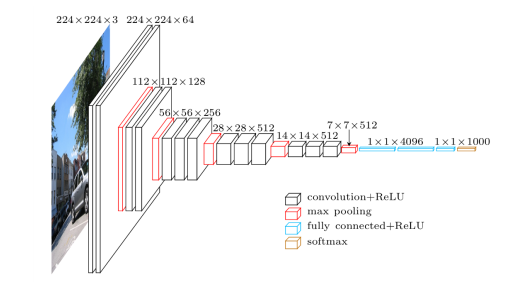
\includegraphics[width=0.6\textwidth]{./figures/VGGNet}
\caption{VGG Net Architecture}
\end{figure}
This architecture was introduced by the researchers at Visual Graphics Group at Oxford (hence the name VGG).
The architecture is characterized by it's pyramidal shape, where the bottom layers which are closer to the image are wide, whereas the top layers are deep.


\subsection[ResNet]{ResNet}

Residual Networks (ResNet in short) consists of multiple subsequent residual modules, which are the basic building block of ResNet architecture. A representation of residual module is as follows.


\begin{figure}[H]
\centering
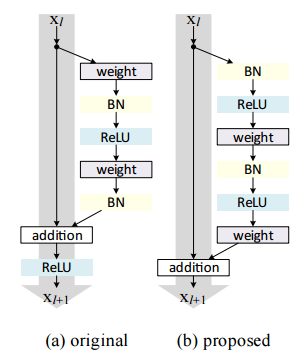
\includegraphics[width=0.4\textwidth]{./figures/ResNet}
\caption{ResNet Architecture}
\end{figure}

The main advantage of ResNet is that hundreds, even thousands of these residual layers can be used to create a network and then trained. This is a bit different from usual sequential networks, where you see that there is reduced performance upgrades as you increase the number of layers.


